\pgfsetplotmarksize{0pt}
\begin{figure}
 \centering
 \caption{\label{CBCvsMSTAV-01sEV100K30}CBCvsMSTAV-01sEV100K30},
 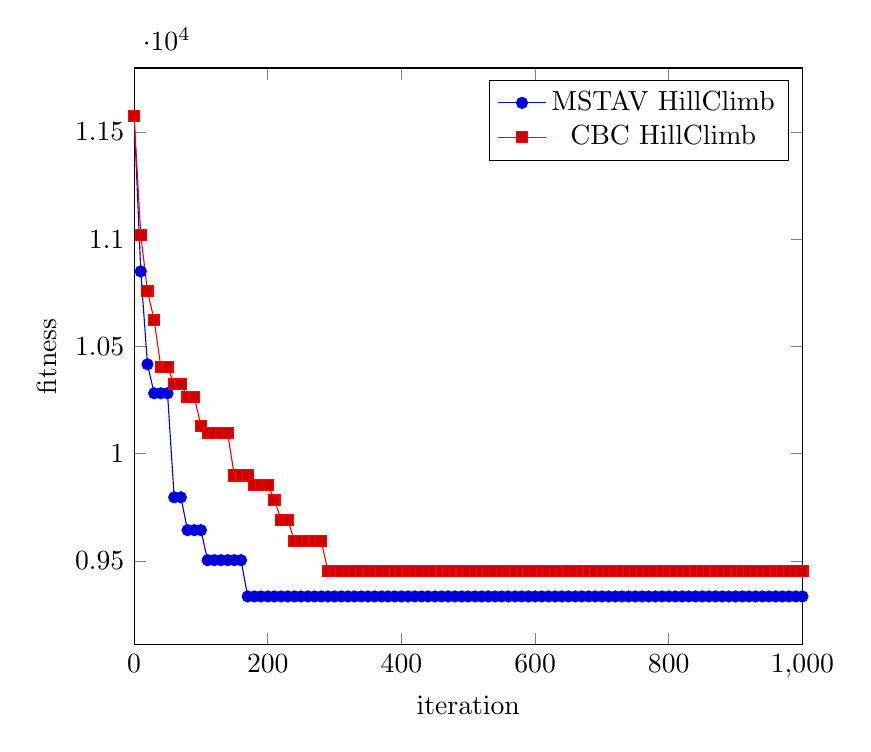
\begin{tikzpicture}
 \begin{axis}[
   width=0.7\textwidth,
   scale only axis,
   xlabel=iteration,
   ylabel=fitness,
   xmin=0,xmax=1000,
   domain=0:1000]
   \addplot coordinates {
     (0,11574)
     (10,10850)
     (20,10417)
     (30,10282)
     (40,10282)
     (50,10282)
     (60,9797)
     (70,9797)
     (80,9644)
     (90,9644)
     (100,9644)
     (110,9504)
     (120,9504)
     (130,9504)
     (140,9504)
     (150,9504)
     (160,9504)
     (170,9335)
     (180,9335)
     (190,9335)
     (200,9335)
     (210,9335)
     (220,9335)
     (230,9335)
     (240,9335)
     (250,9335)
     (260,9335)
     (270,9335)
     (280,9335)
     (290,9335)
     (300,9335)
     (310,9335)
     (320,9335)
     (330,9335)
     (340,9335)
     (350,9335)
     (360,9335)
     (370,9335)
     (380,9335)
     (390,9335)
     (400,9335)
     (410,9335)
     (420,9335)
     (430,9335)
     (440,9335)
     (450,9335)
     (460,9335)
     (470,9335)
     (480,9335)
     (490,9335)
     (500,9335)
     (510,9335)
     (520,9335)
     (530,9335)
     (540,9335)
     (550,9335)
     (560,9335)
     (570,9335)
     (580,9335)
     (590,9335)
     (600,9335)
     (610,9335)
     (620,9335)
     (630,9335)
     (640,9335)
     (650,9335)
     (660,9335)
     (670,9335)
     (680,9335)
     (690,9335)
     (700,9335)
     (710,9335)
     (720,9335)
     (730,9335)
     (740,9335)
     (750,9335)
     (760,9335)
     (770,9335)
     (780,9335)
     (790,9335)
     (800,9335)
     (810,9335)
     (820,9335)
     (830,9335)
     (840,9335)
     (850,9335)
     (860,9335)
     (870,9335)
     (880,9335)
     (890,9335)
     (900,9335)
     (910,9335)
     (920,9335)
     (930,9335)
     (940,9335)
     (950,9335)
     (960,9335)
     (970,9335)
     (980,9335)
     (990,9335)
     (1000,9335)
   };
   \addlegendentry{MSTAV HillClimb}
   \addplot coordinates {
     (0,11574)
     (10,11020)
     (20,10758)
     (30,10624)
     (40,10405)
     (50,10405)
     (60,10324)
     (70,10324)
     (80,10265)
     (90,10265)
     (100,10130)
     (110,10095)
     (120,10095)
     (130,10095)
     (140,10095)
     (150,9899)
     (160,9899)
     (170,9899)
     (180,9856)
     (190,9856)
     (200,9856)
     (210,9786)
     (220,9690)
     (230,9690)
     (240,9595)
     (250,9595)
     (260,9595)
     (270,9595)
     (280,9595)
     (290,9454)
     (300,9454)
     (310,9454)
     (320,9454)
     (330,9454)
     (340,9454)
     (350,9454)
     (360,9454)
     (370,9454)
     (380,9454)
     (390,9454)
     (400,9454)
     (410,9454)
     (420,9454)
     (430,9454)
     (440,9454)
     (450,9454)
     (460,9454)
     (470,9454)
     (480,9454)
     (490,9454)
     (500,9454)
     (510,9454)
     (520,9454)
     (530,9454)
     (540,9454)
     (550,9454)
     (560,9454)
     (570,9454)
     (580,9454)
     (590,9454)
     (600,9454)
     (610,9454)
     (620,9454)
     (630,9454)
     (640,9454)
     (650,9454)
     (660,9454)
     (670,9454)
     (680,9454)
     (690,9454)
     (700,9454)
     (710,9454)
     (720,9454)
     (730,9454)
     (740,9454)
     (750,9454)
     (760,9454)
     (770,9454)
     (780,9454)
     (790,9454)
     (800,9454)
     (810,9454)
     (820,9454)
     (830,9454)
     (840,9454)
     (850,9454)
     (860,9454)
     (870,9454)
     (880,9454)
     (890,9454)
     (900,9454)
     (910,9454)
     (920,9454)
     (930,9454)
     (940,9454)
     (950,9454)
     (960,9454)
     (970,9454)
     (980,9454)
     (990,9454)
     (1000,9454)
   };
   \addlegendentry{CBC HillClimb}
 \end{axis}
 \end{tikzpicture}
\end{figure}
